\chapter{从粒子力学到经典场}

\section{什么是场}

上一讲从不变作用量出发发展了相对论性粒子力学。现在我们改变动力学对象。本讲的主题是经典场论，而不是量子场论。量子力学偶尔会提供一个有用的对照，但本章的方程描述的是普通的经典场。电磁学是背景中熟悉的模型：电磁波在空间中传播并与带电粒子相互作用。我们从一个更为简单的场开始。

一个时空可以有许多空间坐标，但它只有一个时间坐标。写
\begin{equation}
x^\mu=(t,x^1,\ldots,x^d),
\end{equation}
其中空间指标 \(i=1,\ldots,d\)。数 \(d\) 可以是三，正如我们的世界那样，也可以是一、二、九、二十五，或模型中任何其他有用的数。在这个阶段，重要的不对称性在于仍然只有一个时间方向。本讲并不试图解释为什么具有多个时间的理论如此困难；它只是采用普通因果物理得以表述的单时间框架。

场是一种可测量的量，其值可以随地点和时间而变化。温度是一个简单的例子：
\begin{equation}
T=T(\mathbf{x},t).
\end{equation}
它为每一个事件赋予一个数，因此它是一个标量场。风速也随空间和时间变化，但它有大小和方向，因而有多个分量；它是一个矢量场。在相对论物理中，自然的矢量有四个分量而不是三个。

在本讲的大部分内容中，场只有一个分量，并用对应于 \(f\) 的希腊字母表示：
\begin{equation}
\phi=\phi(\mathbf{x},t).
\label{eq:sr4-field-definition}
\end{equation}
称 \(\phi\) 为标量，最终将意味着比说它有一个分量更多的东西。它将意味着所有惯性观测者在同一物理事件处为 \(\phi\) 赋予相同的值。这一变换律只有在变分力学建立之后才会进入。

\section{粒子原型}

\subsection{一个称为\texorpdfstring{\(\phi\)}{phi}的坐标}

通往场论的最快途径，是从一个普通的非相对论性粒子退回去开始。设粒子在一条直线上运动，但把它的坐标称为 \(\phi\) 而不是 \(x\)。把坐标命名为 \(x\) 并没有数学上的义务；选择这个不寻常的名称是为了使即将到来的类比变得可见。水平地画出时间。粒子的整个历史于是是一条曲线 \(\phi(t)\)，它可以经过正值和负值。

对于固定的初始和最终时刻 \(a\) 和 \(b\)，作用量为
\begin{align}
A[\phi]
&=\int_a^b dt\,L(\phi,\dot\phi),\\
L(\phi,\dot\phi)
&=\frac{m}{2}\dot\phi^{\,2}-V(\phi).
\label{eq:sr4-particle-lagrangian}
\end{align}
欧拉--拉格朗日方程为
\begin{equation}
\frac{d}{dt}\left(\frac{\partial L}{\partial\dot\phi}\right)
-\frac{\partial L}{\partial\phi}=0.
\label{eq:sr4-particle-el}
\end{equation}
对于 \eqref{eq:sr4-particle-lagrangian} 中的拉格朗日量，
\begin{equation}
\frac{\partial L}{\partial\dot\phi}=m\dot\phi,
\qquad
\frac{\partial L}{\partial\phi}=-\frac{dV}{d\phi},
\end{equation}
所以
\begin{equation}
\boxed{m\ddot\phi=-\frac{dV}{d\phi}}.
\label{eq:sr4-newton}
\end{equation}
这不过是牛顿方程，以 \(\phi\) 作为坐标写出。

\begin{figure}[htbp]
\centering
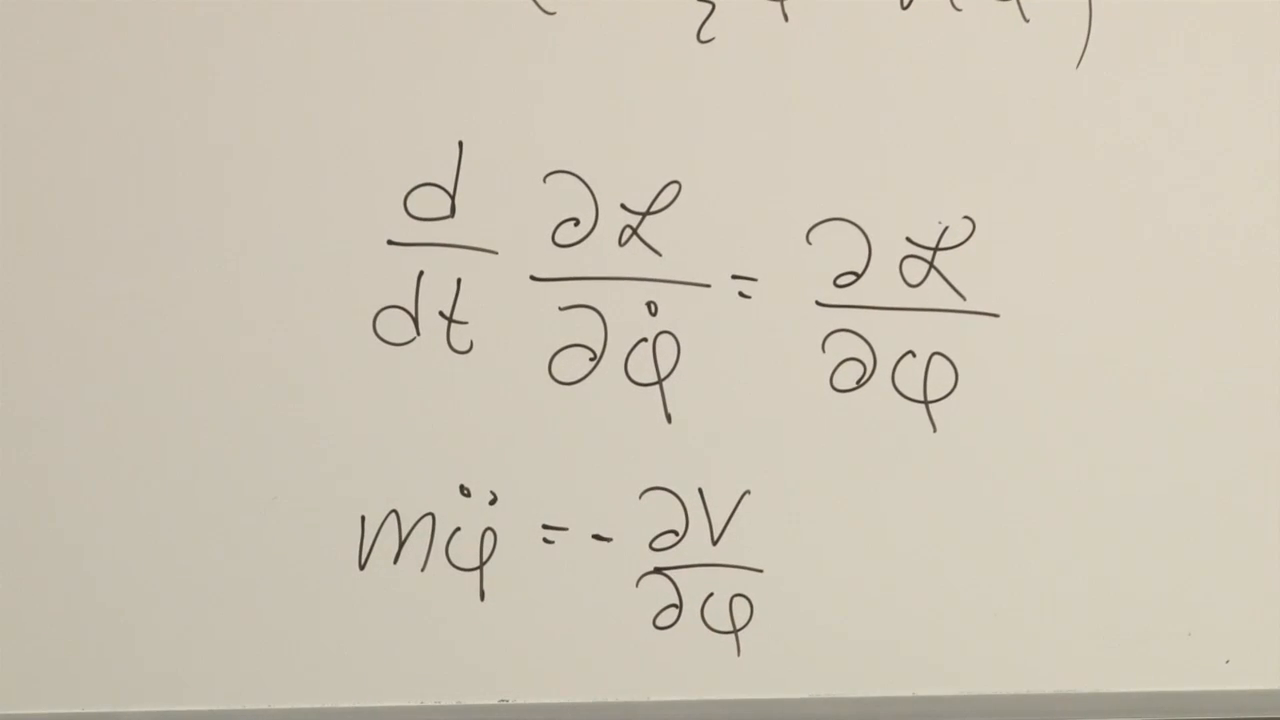
\includegraphics[width=0.90\textwidth]{lecture_04_figure_01.png}
\caption{普通的欧拉--拉格朗日方程及其关于坐标 \(\phi(t)\) 的牛顿结果。}
\lectureframe{00:10:18}
\end{figure}

物理路径在端点保持固定时使作用量取驻值。本讲常说 \emph{极小}，但精确的陈述是驻定性：该路径可以给出极小值、极大值或另一个驻定值。一个有用的心智模型是把时间区间分成许多小段。作用量成为 \(\phi\) 的许多采样值的函数。在保持端点固定的同时移动这些值，并对其中每一个求导，就是欧拉--拉格朗日方程的有限维祖先。

\subsection{作为 \texorpdfstring{\(0+1\)}{0+1} 维理论的力学}

现在想象一个有时间但没有空间维度的世界。它的空间是一个单点。那个世界中的场不能依赖于位置，因为没有位置可供依赖；它只能是一个函数 \(\phi(t)\)。因此，普通的一坐标粒子力学可以被读作 \(0+1\) 维中的场论。数学没有改变。改变的只是解释，从粒子的位置变为一个没有空间的 world 中场之值。

\begin{figure}[htbp]
\centering
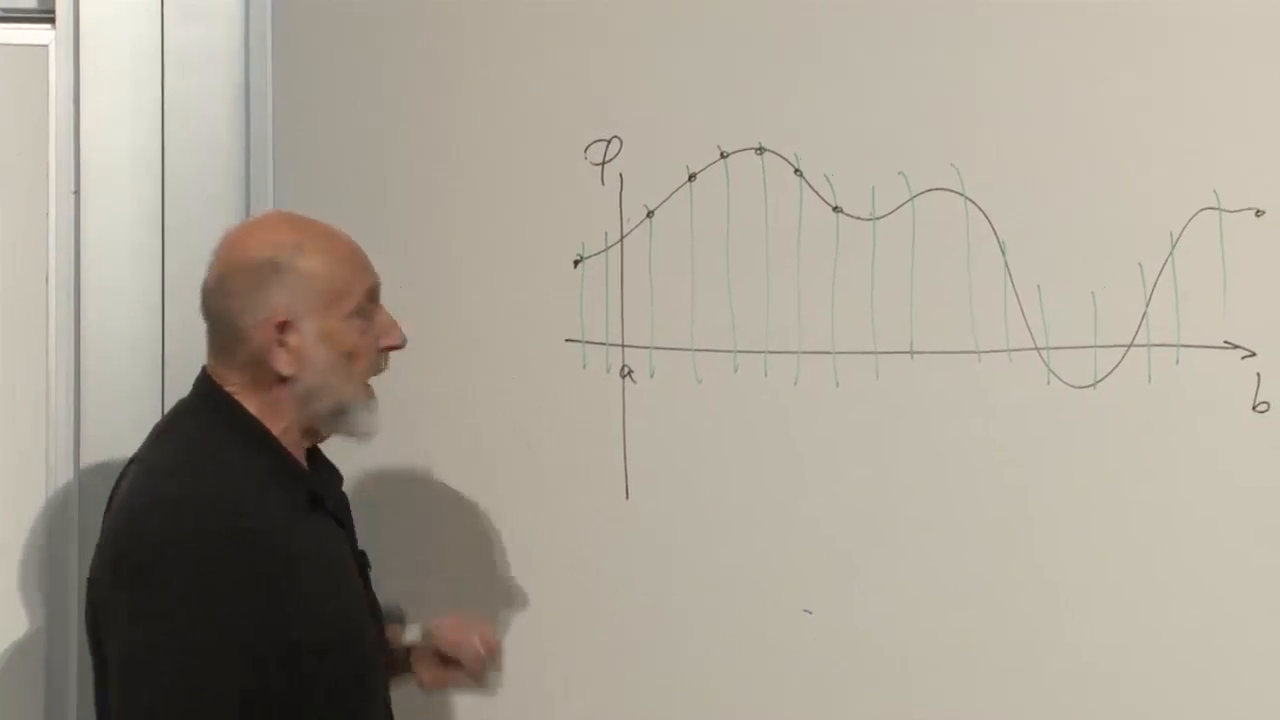
\includegraphics[width=0.90\textwidth]{lecture_04_figure_02.png}
\caption{采样历史 \(\phi(t)\)：一条粒子轨迹，以及在新解释下 \(0+1\) 维中的一段场历史。}
\lectureframe{00:14:30}
\end{figure}

\begin{classroomqa}
\audiencequestion{当没有空间维度时，势会消失吗？}
\lecturerresponse{不会。空间变化消失了，但场仍然有一个值。能量可能通过\(V(\phi)\)依赖于那个值。在粒子解释中，把曲线向上或向下移动会改变势能；在场解释中，\(\phi\)的不同值携带不同的势能。\lecturetimestamp{00:15:00}}
\end{classroomqa}

\begin{classroomqa}
\audiencequestion{与其想象完全没有空间，能否想象一个普通空间，其中场只依赖于时间？}
\lecturerresponse{可以。为此，局部数学是相同的：所有空间导数都为零，只剩下\(\phi(t)\)。称其为\(0+1\)维理论隔离出了那种约化结构，但更大世界中的空间均匀场提供了同样的直观图像。\lecturetimestamp{00:16:25}}
\end{classroomqa}

这段迂回的目的现在清楚了。我们知道一个依赖于一个坐标——时间——的场的作量原理。我们可以用它的模式来猜测一个依赖于时空所有坐标的场的作量原理。

\section{时空上的场历史}

\subsection{从曲线到曲面}

在\(1+1\)维中，时空本身是一个带有坐标\(t\)和\(x\)的平面。值\(\phi(x,t)\)提供了第三个方向。因此，场的历史不是一条曲线，而是时空平面之上的一个曲面。该曲面可以升到零以上或降到零以下，因为标量场不必为正。

\begin{figure}[htbp]
\centering
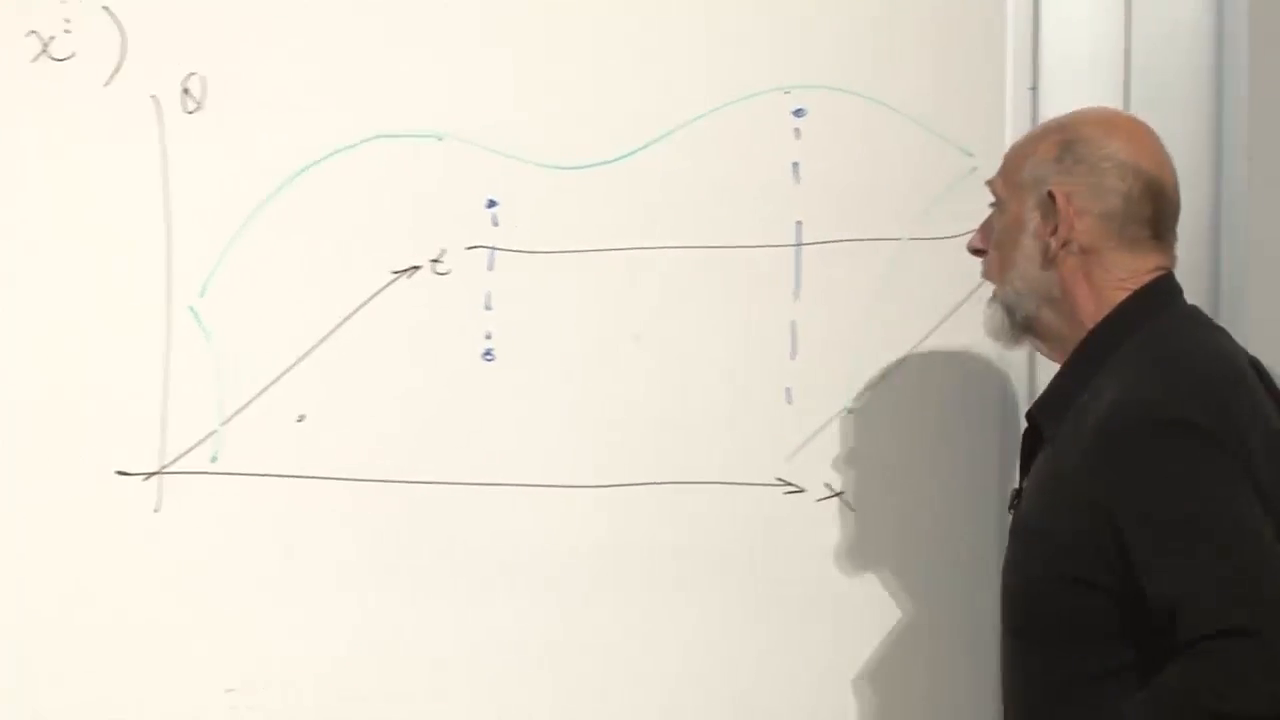
\includegraphics[width=0.90\textwidth]{lecture_04_figure_03.png}
\caption{一个标量场历史，画为\(1+1\)维时空平面之上的曲面。}
\lectureframe{00:20:46}
\end{figure}

我们的物理时空被称为\(3+1\)维：三个空间维度和一个时间维度。桌面模型是\(2+1\)维的，而被约束在导线上的珠子暗示了一个\(1+1\)维世界。绘制\(\phi\)所需的额外轴使得即使\(3+1\)情形也无法忠实画出，但定义是明确的：一个完整的历史为每个时空事件赋予一个\(\phi\)值。

\subsection{从固定端点到固定边界数据}

粒子变分问题固定两个端点，并变化它们之间的曲线。其场论类比选取一个时空区域，固定该区域边界上的\(\phi\)，并变化内部的\(\phi\)。该区域可以是\(1+1\)维绘图中的一个矩形，也可以是更高维时空中任何合适的区域。

\begin{figure}[htbp]
\centering
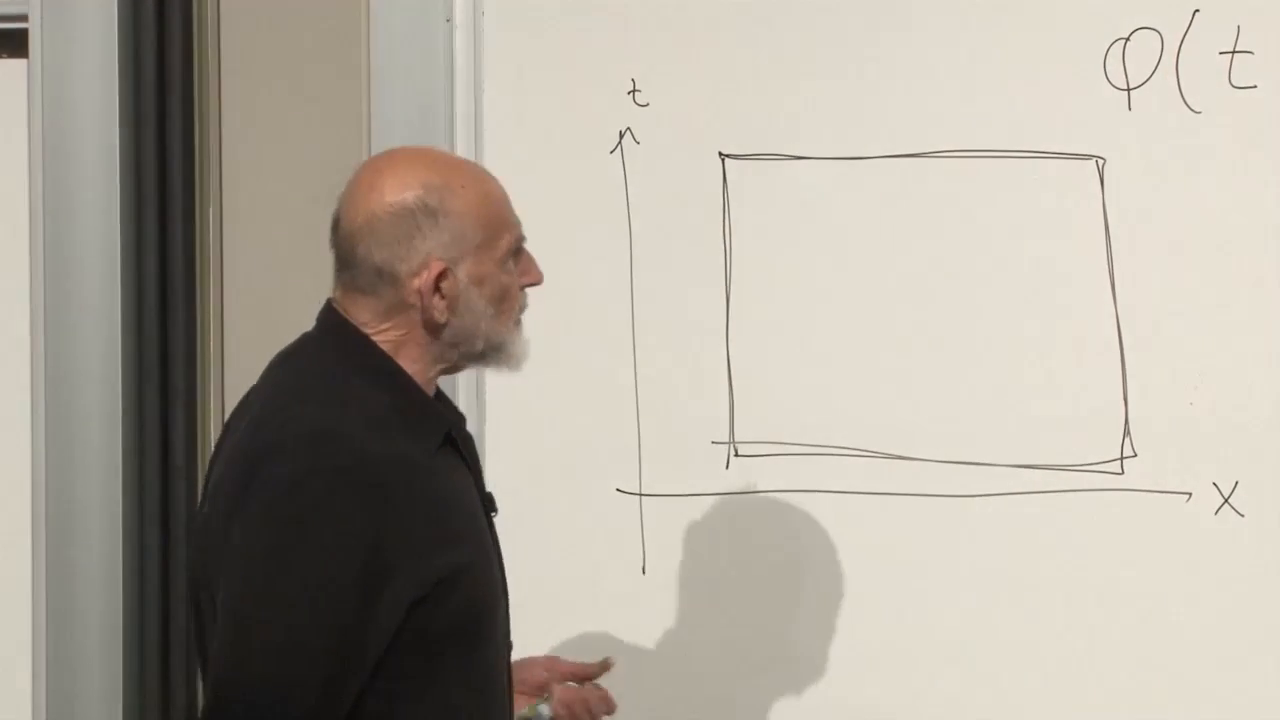
\includegraphics[width=0.90\textwidth]{lecture_04_figure_04.png}
\caption{一个时空区域，其整个边界被固定，而内部的场被变化。}
\lectureframe{00:24:52}
\end{figure}

\begin{classroomqa}
\audiencequestion{当势显式依赖于时间时，拉格朗日表述仍然有效吗？}
\lecturerresponse{有效。欧拉--拉格朗日表述和哈密顿表述仍然有效。一般来说，失去的是能量守恒：显式时间依赖破坏了时间平移对称性。场论中相应的陈述是，显式时空依赖是允许的，尽管它会影响相关的守恒定律。\lecturetimestamp{00:23:49}}
\end{classroomqa}

\begin{classroomqa}
\audiencequestion{对于矩形场区域，是只固定顶部和底部，还是固定整个边界？}
\lecturerresponse{对于这个变分构造，整个边界都被固定：\(1+1\)维矩形中的所有四条边。场只允许在内部摆动。这是粒子力学中固定两个端点的直接类比。\lecturetimestamp{00:24:24}}
\end{classroomqa}

固定整个边界是关于用于推导方程的变分的陈述。当由此得到的双曲型场方程被当作物理演化问题处理时，人们更常会指定适当的初始数据，并让方程将其向前传播。

\section{作用量与场的欧拉--拉格朗日方程}

\subsection{拉格朗日密度}

把时空区域分成小胞元。假设作用量是局部贡献之和，每个胞元贡献一项。在连续极限下，该和变成时空上的积分：
\begin{equation}
A[\phi]
=
\int_{\Omega} d^4x\,
\mathcal{L}\!\left(
\phi,\partial_\mu\phi;x^\mu
\right),
\qquad
d^4x=dt\,dx\,dy\,dz.
\label{eq:sr4-field-action}
\end{equation}
量\(\mathcal{L}\)是拉格朗日密度。\(\mathcal{L}(\phi,\partial_\mu\phi;x^\mu)\)中的分号把动力学变量与可能的显式坐标依赖分开。在均匀封闭系统中，最后这种依赖通常不存在，但变分形式并不禁止它。

紧凑记号
\begin{equation}
\partial_\mu\phi
\equiv
\frac{\partial\phi}{\partial x^\mu}
\end{equation}
把时间导数与空间导数收集在一起。在讲座的分量记号中，也可以改写成
\begin{equation}
\begin{aligned}
\phi_t&=\frac{\partial\phi}{\partial t},\\
\phi_x&=\frac{\partial\phi}{\partial x},\\
\phi_y&=\frac{\partial\phi}{\partial y},\\
\phi_z&=\frac{\partial\phi}{\partial z}.
\end{aligned}
\label{eq:sr4-component-derivatives}
\end{equation}
场可以有若干个，正如一个粒子可以有若干个坐标。眼下只有一个场 \(\phi\)。

符号 \(d^4x\) 只是四维坐标测度的简写。在另一维度的时空中，它会被 \(d^Dx\) 取代。在 \(0+1\) 维的原型中，\(D=1\)，而 \(d^1x\) 就只是 \(dt\)。

\begin{figure}[htbp]
\centering
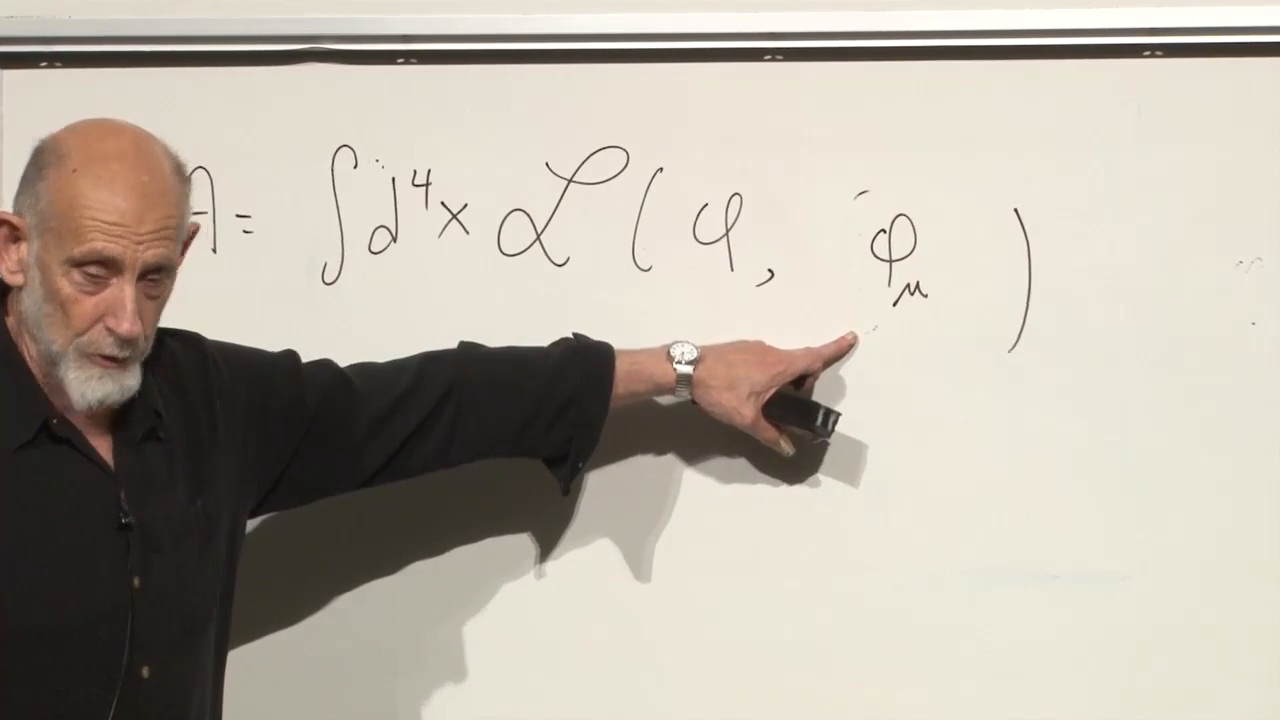
\includegraphics[width=0.90\textwidth]{lecture_04_figure_05.png}
\caption{作用量密度被写成 \(\phi\) 及其时空导数的局域函数。}
\lectureframe{00:32:51}
\end{figure}

\begin{classroomqa}
\audiencequestion{拉格朗日密度是否也可以依赖于 \(x,y,z\) 本身？}
\lecturerresponse{可以，正如粒子拉格朗日量可以显式依赖于 \(t\)。对于平移不变的封闭系统，它通常并不如此，但显式的坐标依赖并不会使这一形式体系失效。\lecturetimestamp{00:30:29}}
\end{classroomqa}

\begin{classroomqa}
\audiencequestion{到目前为止的构造是专门针对标量场的，还是具有一般性？}
\lecturerresponse{到目前为止，变分模式是一般的。只写一个分量暗示着标量场。矢量场或一组场会带有额外的分量标签，而人们要对每一个分量作变分。\lecturetimestamp{00:31:00}}
\end{classroomqa}

\subsection{点阵图像}

在精细的时空点阵上，导数变成相邻场值之间的有限差分。于是作用量成为许多变量的普通函数。一个方向上有十个点、另一个方向上有八个点的网格，就已经给出八十个场变量。细化网格会增加它们的数目，但极小化规则仍然初等：对每个内点的场值求作用量的导数，并令结果为零。

\begin{figure}[htbp]
\centering
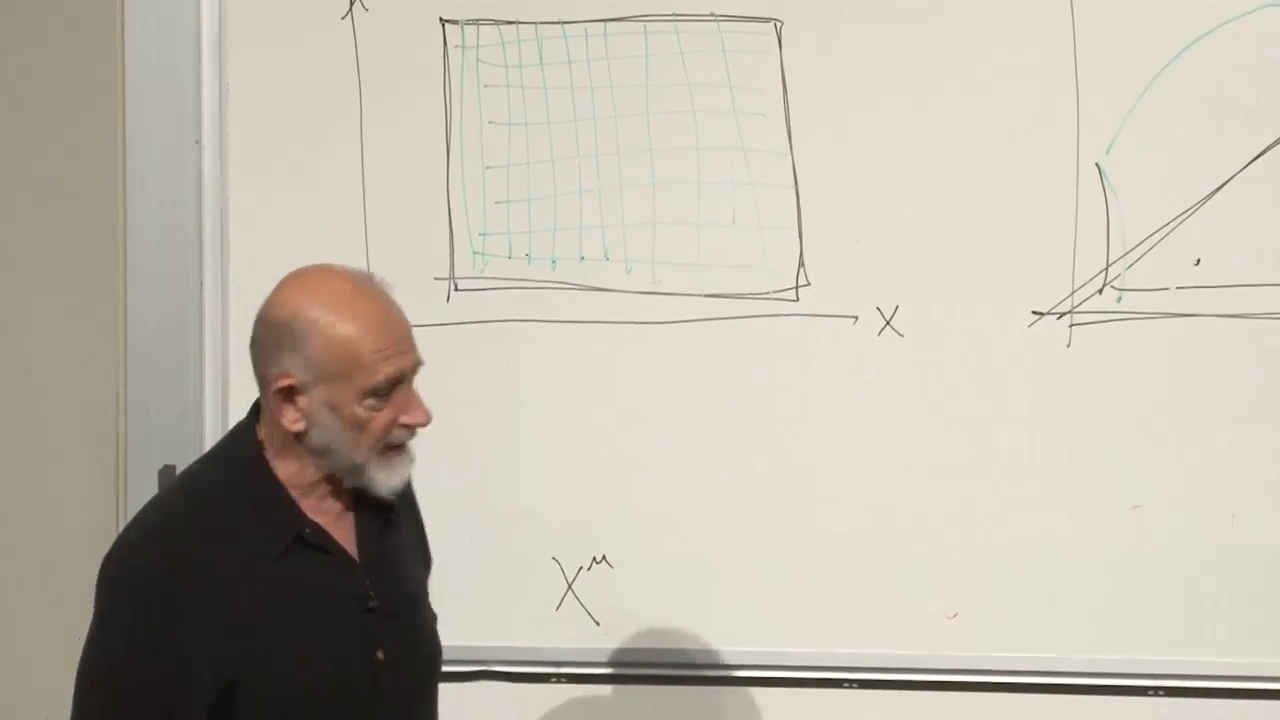
\includegraphics[width=0.90\textwidth]{lecture_04_figure_06.png}
\caption{时空区域被划分成胞元，使得在连续极限之前，作用量成为普通的多元函数。}
\lectureframe{00:34:05}
\end{figure}

取连续极限便得到场的欧拉--拉格朗日方程，
\begin{equation}
\boxed{
\partial_\mu
\left[
\frac{\partial\mathcal{L}}
{\partial(\partial_\mu\phi)}
\right]
-
\frac{\partial\mathcal{L}}{\partial\phi}
=0
}.
\label{eq:sr4-field-el}
\end{equation}
重复的 \(\mu\) 对所有时空方向求和。不写成求和简记，同一个方程是
\begin{align}
&
\frac{\partial}{\partial t}
\left(\frac{\partial\mathcal{L}}{\partial\phi_t}\right)
+
\frac{\partial}{\partial x}
\left(\frac{\partial\mathcal{L}}{\partial\phi_x}\right)
+
\frac{\partial}{\partial y}
\left(\frac{\partial\mathcal{L}}{\partial\phi_y}\right)
\nonumber\\
&\hspace{3em}
+
\frac{\partial}{\partial z}
\left(\frac{\partial\mathcal{L}}{\partial\phi_z}\right)
-
\frac{\partial\mathcal{L}}{\partial\phi}
=0.
\label{eq:sr4-field-el-expanded}
\end{align}
第一项是熟悉的粒子项。场论为每一个空间方向添加一个类似的项。最后一项，
\(-\partial\mathcal{L}/\partial\phi\)，保持不变。

\begin{figure}[htbp]
\centering
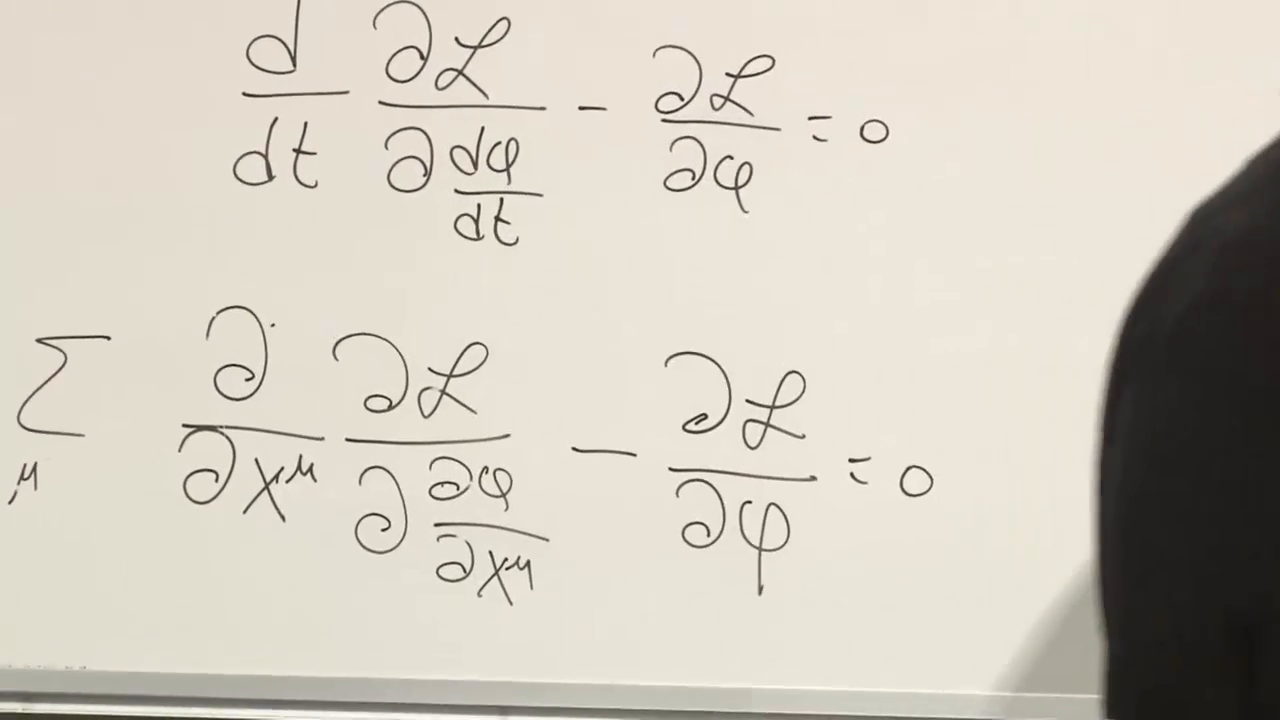
\includegraphics[width=0.90\textwidth]{lecture_04_figure_07.png}
\caption{一维欧拉--拉格朗日方程及其时空推广，上下并列写出。}
\lectureframe{00:38:44}
\end{figure}

这一主题也称为连续介质力学。取决于自由度，同样的数学可以描述流体流动、弹性位移，或另一种连续介质。

\begin{classroomqa}
\audiencequestion{同样的方程在一个有空间但没有时间的世界里会成立吗？}
\lecturerresponse{会，作为一个纯空间的变分问题。在物理上，这正是人们寻找静态解的方式：假定场不依赖于时间，丢弃所有时间导数，并求解剩下的空间方程。一个不依赖于时间的电场或磁场位形就是一个例子。\lecturetimestamp{00:40:05}}
\end{classroomqa}

\section{猜测最简单的标量动力学}

\subsection{为什么符号不能全都相同}

回到粒子动能项 \(\tfrac12\dot\phi^2\)，把它无关紧要的整体系数设为 1，并试着将它推广。第一个猜测可能是
\begin{equation}
\mathcal{L}_{+}
=
\frac12
\left[
\phi_t^2+\phi_x^2+\phi_y^2+\phi_z^2
\right].
\label{eq:sr4-all-plus}
\end{equation}
这是一次有用的错误转向。它以完全相同的符号对待时间和空间。由此得到的方程不会具有波传播的双曲结构。正确的相对论性组合对时间取一个符号，对空间取相反的符号。

\begin{classroomqa}
\audiencequestion{全正号的表达式之所以错误，是因为拉格朗日量应当具有相对论不变性吗？}
\lecturerresponse{这是更深刻的答案，而且它是正确的。讲座首先以更朴素的方式得到符号：波把时间中的演化与空间中的变化区分开来，所以时间不能完全像另一个空间坐标那样进入。洛伦兹不变性很快就会把这一直觉变成一条精确的规则。\lecturetimestamp{00:43:19}}
\end{classroomqa}

恢复一个特征速率 \(c\)，简单的标量拉格朗日密度是
\begin{equation}
\boxed{
\mathcal{L}
=
\frac12
\left[
\frac{1}{c^2}\phi_t^2
-\phi_x^2-\phi_y^2-\phi_z^2
\right]
-V(\phi)
}.
\label{eq:sr4-scalar-lagrangian}
\end{equation}
对于相对论场，\(c\) 是光速。在连续介质模型中，它也可以是声速、弹性波的速率，或另一种特征传播速率。

整体因子 \(1/2\) 是约定俗成的，正如在 \(\tfrac12m\dot\phi^2\) 中那样。将整个作用量乘以一个非零常数不会改变其驻定路径；该约定确定了方程中参数如何命名与归一化。一旦选定了这种归一化，就必须一致地使用它。

\begin{classroomqa}
\audiencequestion{空间梯度项可以被视为势能的一部分吗？}
\lecturerresponse{可以。在动能减势能的组织方式中，动能部分包含时间导数。不含时间导数的项，包括空间梯度和 \(V(\phi)\)，属于势能一侧。在相对论理论中，它们相对符号的最终原因是洛伦兹度规。\lecturetimestamp{00:45:37}}
\end{classroomqa}

\subsection{波动方程}

应用 \eqref{eq:sr4-field-el}。导数项为
\begin{equation}
\frac{\partial\mathcal{L}}{\partial\phi_t}
=\frac{1}{c^2}\phi_t,
\qquad
\frac{\partial\mathcal{L}}{\partial\phi_i}
=-\phi_i,
\end{equation}
而
\begin{equation}
\frac{\partial\mathcal{L}}{\partial\phi}
=-\frac{dV}{d\phi}.
\end{equation}
因此
\begin{equation}
\begin{aligned}
&\boxed{
\frac{1}{c^2}\frac{\partial^2\phi}{\partial t^2}
-\nabla^2\phi
+\frac{dV}{d\phi}
=0
},\\[0.5em]
\nabla^2
&=
\frac{\partial^2}{\partial x^2}
+\frac{\partial^2}{\partial y^2}\\
&\quad
+\frac{\partial^2}{\partial z^2}.
\end{aligned}
\label{eq:sr4-general-scalar-eom}
\end{equation}

若 \(V=0\)，则此式化为
\begin{equation}
\boxed{
\frac{1}{c^2}\phi_{tt}-\nabla^2\phi=0
},
\label{eq:sr4-wave-equation}
\end{equation}
即波动方程。讲座识别出了该方程，但推迟求解。其解以速率 \(c\) 传播扰动。

\begin{figure}[htbp]
\centering
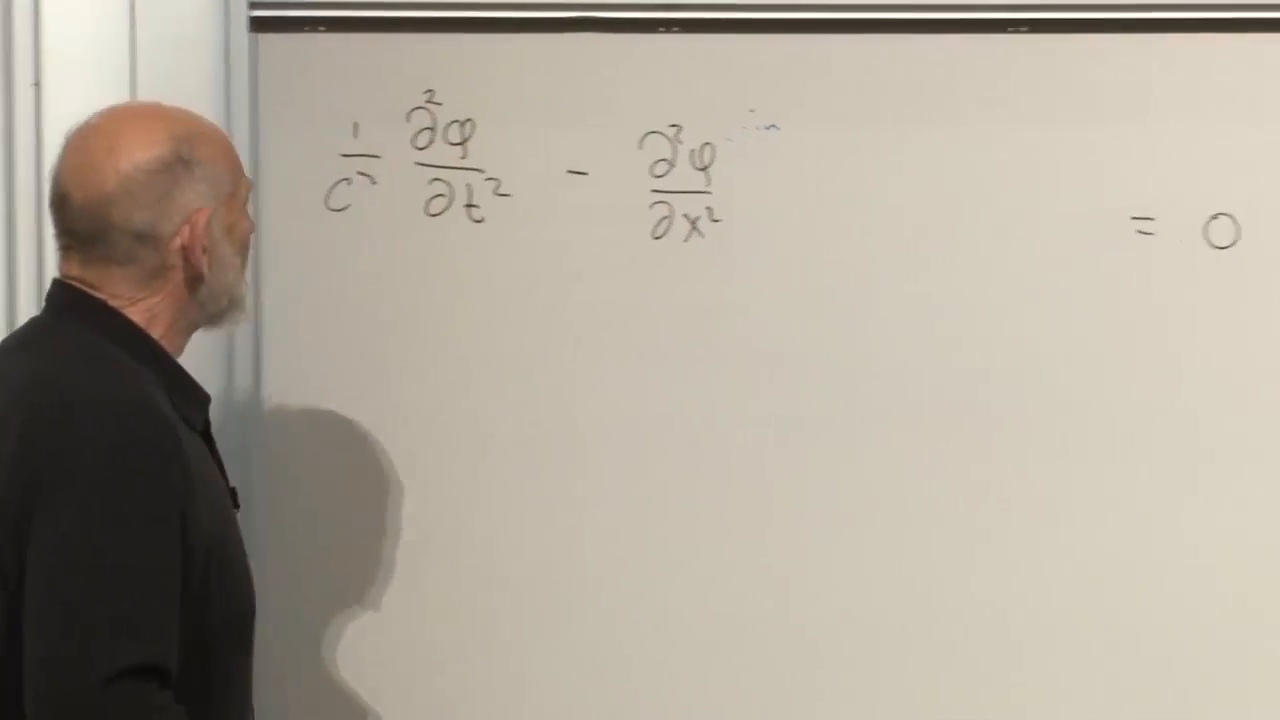
\includegraphics[width=0.90\textwidth]{lecture_04_figure_08.png}
\caption{一维形式 \(c^{-2}\phi_{tt}-\phi_{xx}=0\)，被识别为波动方程。}
\lectureframe{00:50:30}
\end{figure}

\subsection{耦合谐振子场}

现在选择一个二次势，
\begin{equation}
V(\phi)=\frac12\mu^2\phi^2,
\qquad
\frac{dV}{d\phi}=\mu^2\phi.
\label{eq:sr4-quadratic-potential}
\end{equation}
如果 \(\phi\) 是一个粒子的位置，这将是弹簧常数为 \(\mu^2\) 的谐振子的势。对于场，
\begin{equation}
\boxed{
\frac{1}{c^2}\phi_{tt}-\nabla^2\phi+\mu^2\phi=0
}.
\label{eq:sr4-klein-gordon}
\end{equation}
没有空间导数时，这不过是加速度加上常数乘以位移等于零。梯度将相邻点耦合起来，把振子变成承载波动的连续介质。在相对论场论中，\eqref{eq:sr4-klein-gordon} 被称为有质量克莱因--戈登方程；经典地，\(\mu\) 是修正波传播的逆长度标度。

\begin{figure}[htbp]
\centering
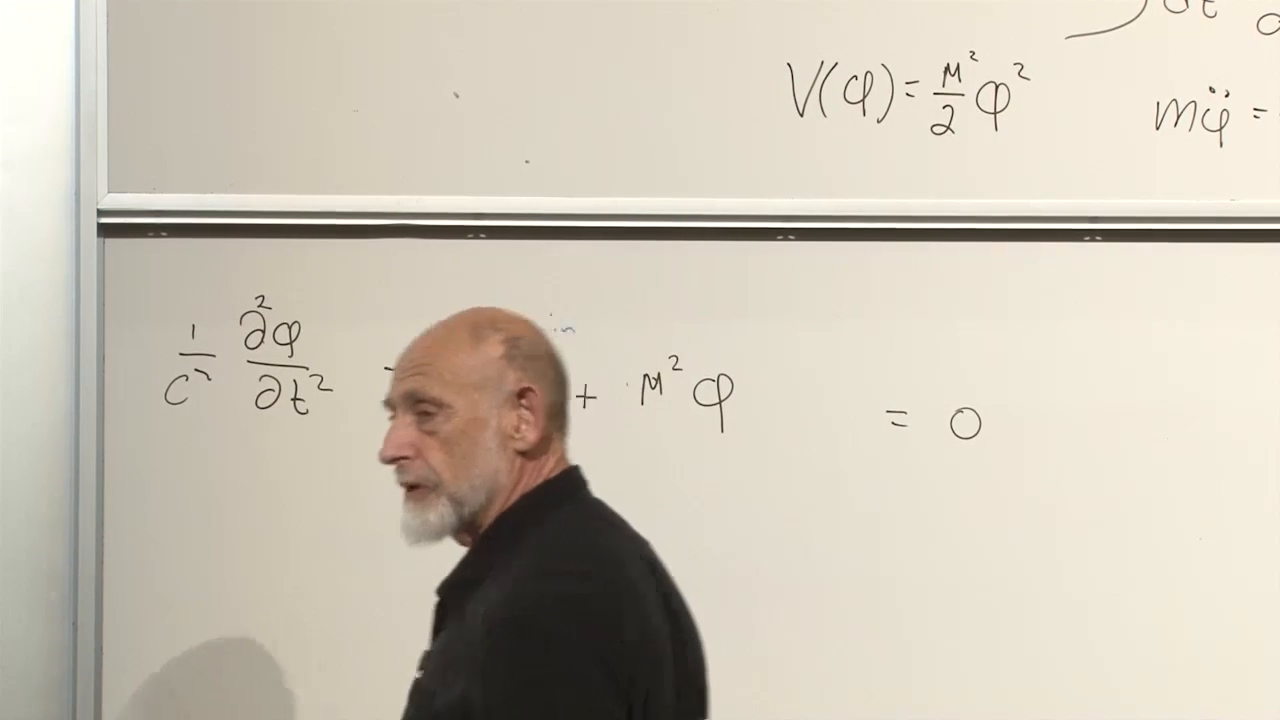
\includegraphics[width=0.90\textwidth]{lecture_04_figure_09.png}
\caption{二次势以及由此得到的带恢复项 \(\mu^2\phi\) 的波动方程。}
\lectureframe{00:52:38}
\end{figure}

\begin{classroomqa}
\audiencequestion{为什么 \(V=\tfrac12\mu^2\phi^2\) 中的因子 \(1/2\) 在运动方程中消失了？}
\lecturerresponse{对 \(\phi^2\) 求导会给出一个因子二。约定性的 \(1/2\) 正是为了使 \(dV/d\phi=\mu^2\phi\)，正如 \(V(x)=\tfrac12kx^2\) 给出恢复力 \(-kx\) 一样。\lecturetimestamp{00:53:17}}
\end{classroomqa}

该方程是线性的：\(\phi\) 及其各阶导数都只出现一次幂。运动方程中诸如 \(\phi^2\) 或 \(\phi\,\partial_\mu\phi\) 的项会使动力学变为非线性。

\section{洛伦兹标量与四维矢量}

\subsection{作用量必须与参考系无关}

仅凭变分机制就可以定义许多可能的场论。相对论施加了额外的要求：作用量在每个惯性系中必须具有相同的值和形式。对于自由粒子，这是通过沿世界线积分不变固有时间 \(d\tau\) 来实现的。对于场，作用量在时空上积分，因此其局部构件必须按适当方式变换。

在固有洛伦兹变换下，时空测度不变，\(d^4x'=d^4x\)。因此，只需要求拉格朗日密度为洛伦兹标量：
\begin{equation}
\mathcal{L}'(x')=\mathcal{L}(x).
\label{eq:sr4-lagrangian-scalar}
\end{equation}

\subsection{标量场}

标量场满足
\begin{equation}
\boxed{\phi'(x')=\phi(x)}.
\label{eq:sr4-scalar-transform}
\end{equation}
坐标 \(x\) 和 \(x'\) 在两个参考系中标示同一事件。观察者所使用的函数表达式可能看起来不同，但赋予该物理事件的数值是相同的。

\begin{figure}[htbp]
\centering
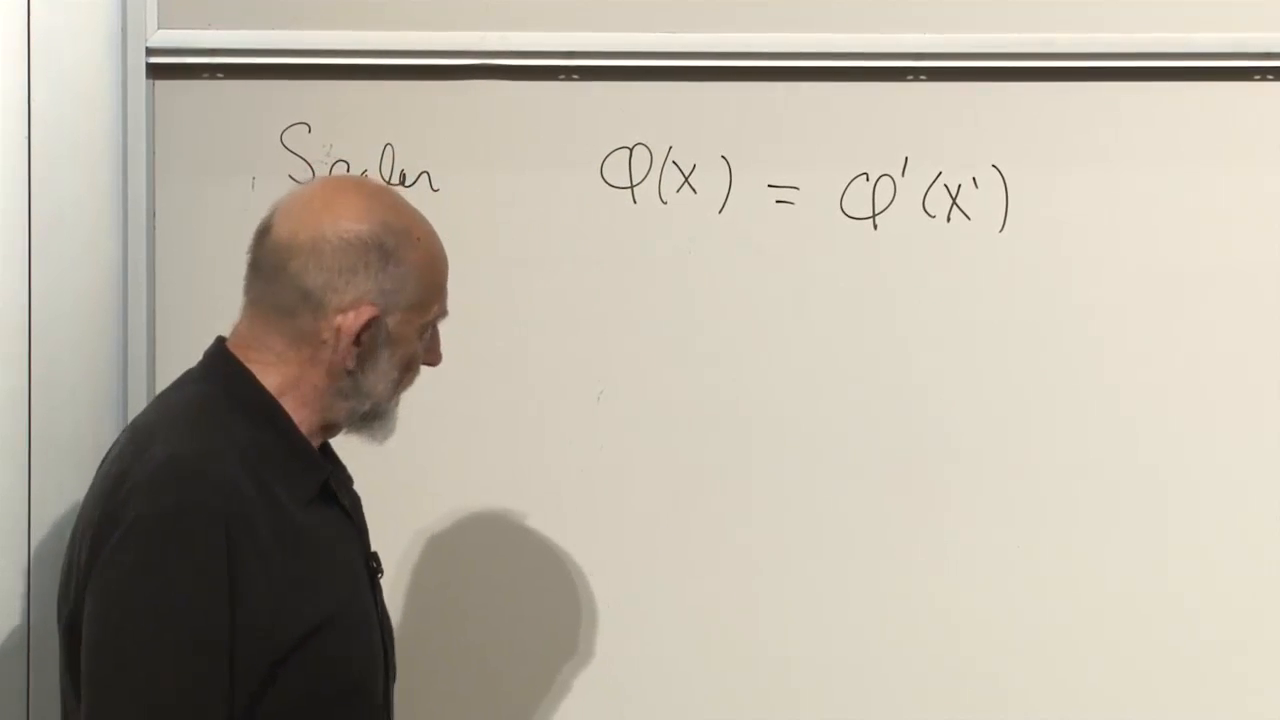
\includegraphics[width=0.90\textwidth]{lecture_04_figure_10.png}
\caption{标量场的定义性变换律：\(\phi(x)=\phi'(x')\)。}
\lectureframe{00:59:33}
\end{figure}

温度提供了早期的直觉，尽管在物质介质中运动的温度计并不是一个完美的相对论例子。重要的是定义 \eqref{eq:sr4-scalar-transform}，而不是温度计的类比。

\subsection{四维矢量}

在单位 \(c=1\) 下，沿 \(x\) 轴以速率 \(v\) 的助推作用为
\begin{equation}
\begin{aligned}
t'&=\gamma(t-vx),\\
x'&=\gamma(x-vt),\\
y'&=y,\\
z'&=z,\\
\gamma&=\frac{1}{\sqrt{1-v^2}}.
\end{aligned}
\label{eq:sr4-x-boost}
\end{equation}

\begin{figure}[htbp]
\centering
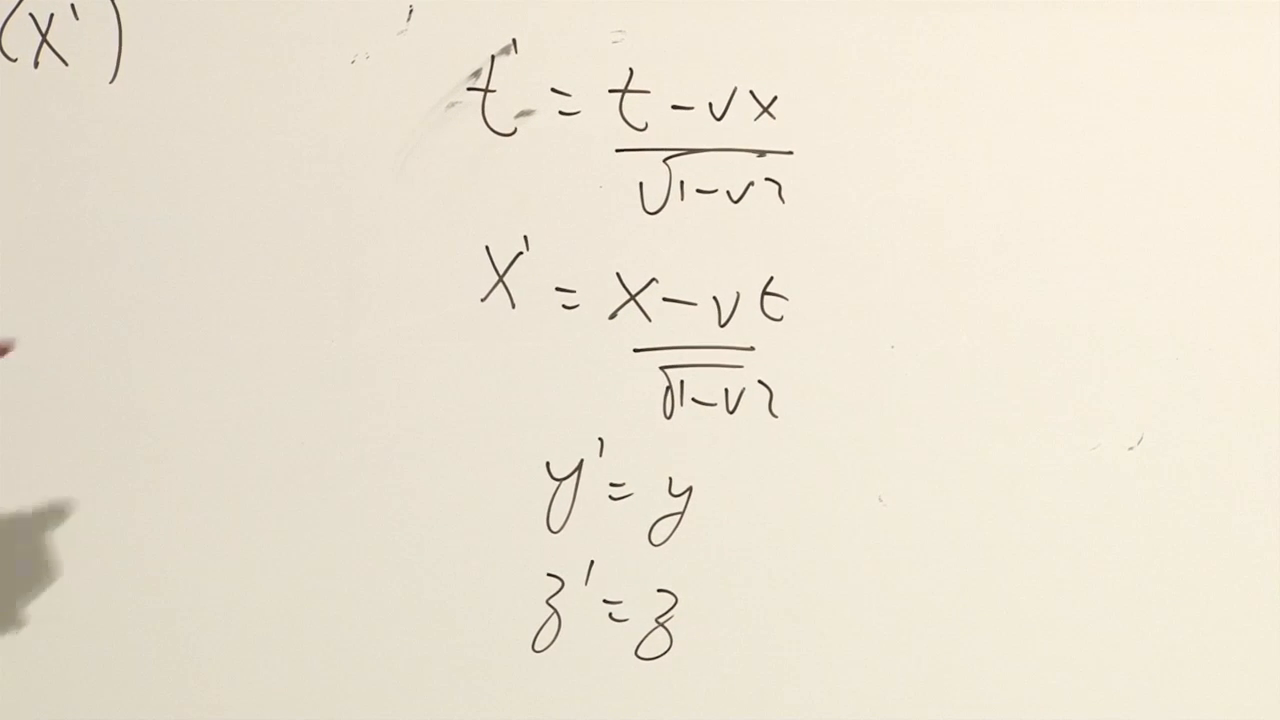
\includegraphics[width=0.90\textwidth]{lecture_04_figure_11.png}
\caption{在 \(c=1\) 单位下沿 \(x\) 轴助推的洛伦兹变换。}
\lectureframe{01:02:26}
\end{figure}

任何在助推下以相同方式混合的四个量构成一个四维矢量。已经遇到的例子有 \(x^\mu\)、\(dx^\mu\) 以及四维速度 \(u^\mu=dx^\mu/d\tau\)。四维矢量乘以标量得到另一个四维矢量。流动的相对论流体提供了一个场值例子：其四维速度 \(u^\mu(x)\) 可以逐事件不同。

对于与 \eqref{eq:sr4-x-boost} 中相同的助推，一个一般四维矢量满足
\begin{equation}
\begin{aligned}
A'^0&=\gamma(A^0-vA^x),\\
A'^x&=\gamma(A^x-vA^0),\\
A'^y&=A^y,\\
A'^z&=A^z.
\end{aligned}
\label{eq:sr4-vector-boost}
\end{equation}

对于一般的四维矢量 \(A^\mu=(A^0,A^x,A^y,A^z)\)，洛伦兹范数
\begin{equation}
\boxed{
A_\mu A^\mu
=(A^0)^2-(A^x)^2-(A^y)^2-(A^z)^2
}
\label{eq:sr4-vector-norm}
\end{equation}
是一个标量。它之所以不变，与
\begin{equation}
d\tau^2=dt^2-dx^2-dy^2-dz^2
\end{equation}
之所以不变的代数理由相同。讲义在为一般矢量寻找尚未用过的字母时一度捉襟见肘，随后接受了 \(A\)，这得益于有人建议用箭头表示 \(A\)。

\begin{figure}[htbp]
\centering
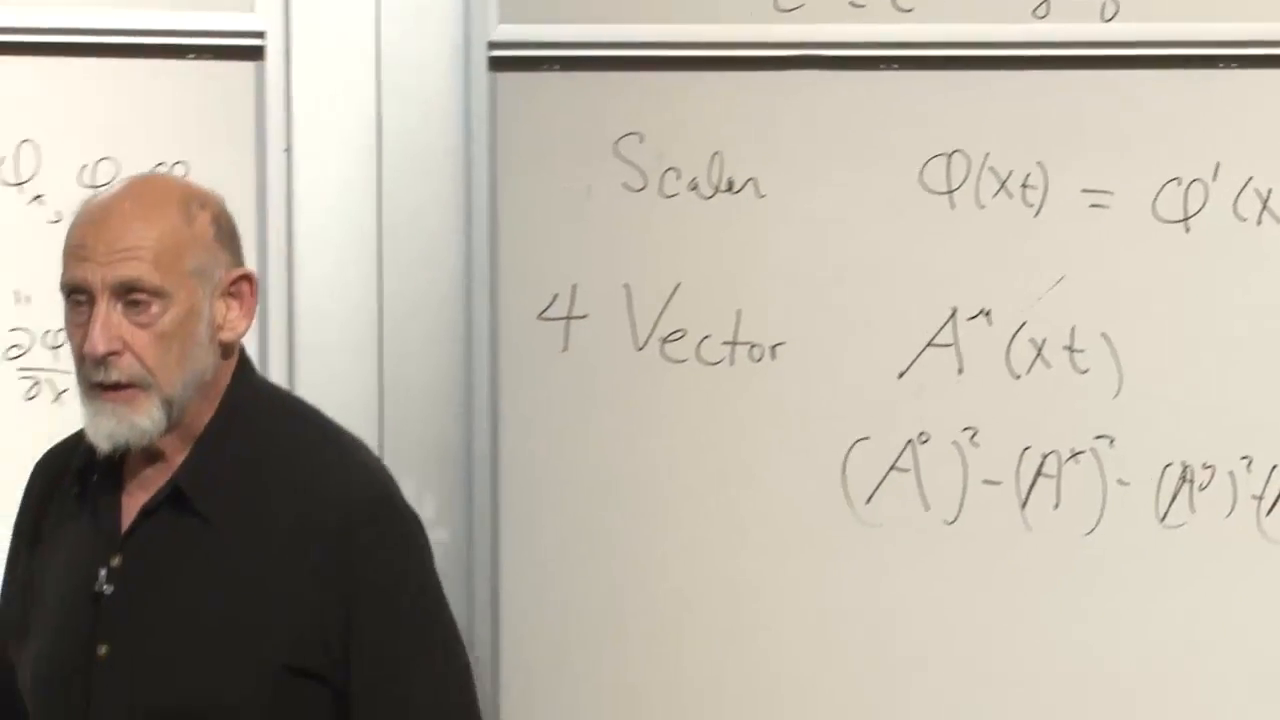
\includegraphics[width=0.90\textwidth]{lecture_04_figure_12.png}
\caption{一般的四维矢量场，以及由它构造不变范数所用的洛伦兹平方差。}
\lectureframe{01:09:06}
\end{figure}

\subsection{标量的导数}

将标量对四个时空坐标求导，得到四个分量
\begin{equation}
\partial_\mu\phi
=
\left(
\frac{\partial\phi}{\partial t},
\frac{\partial\phi}{\partial x},
\frac{\partial\phi}{\partial y},
\frac{\partial\phi}{\partial z}
\right)
\qquad(c=1).
\end{equation}
严格地说，\(\partial_\mu\phi\) 是一个余矢量；闵可夫斯基度规将其指标升高，从而得到 \(\partial^\mu\phi\)。这一区分在此处的分量论证中无关紧要，但它明确地确定了缩并：
\begin{equation}
\boxed{
\partial_\mu\phi\,\partial^\mu\phi
=
\frac{1}{c^2}\phi_t^2
-\phi_x^2-\phi_y^2-\phi_z^2
}.
\label{eq:sr4-derivative-scalar}
\end{equation}

\begin{figure}[htbp]
\centering
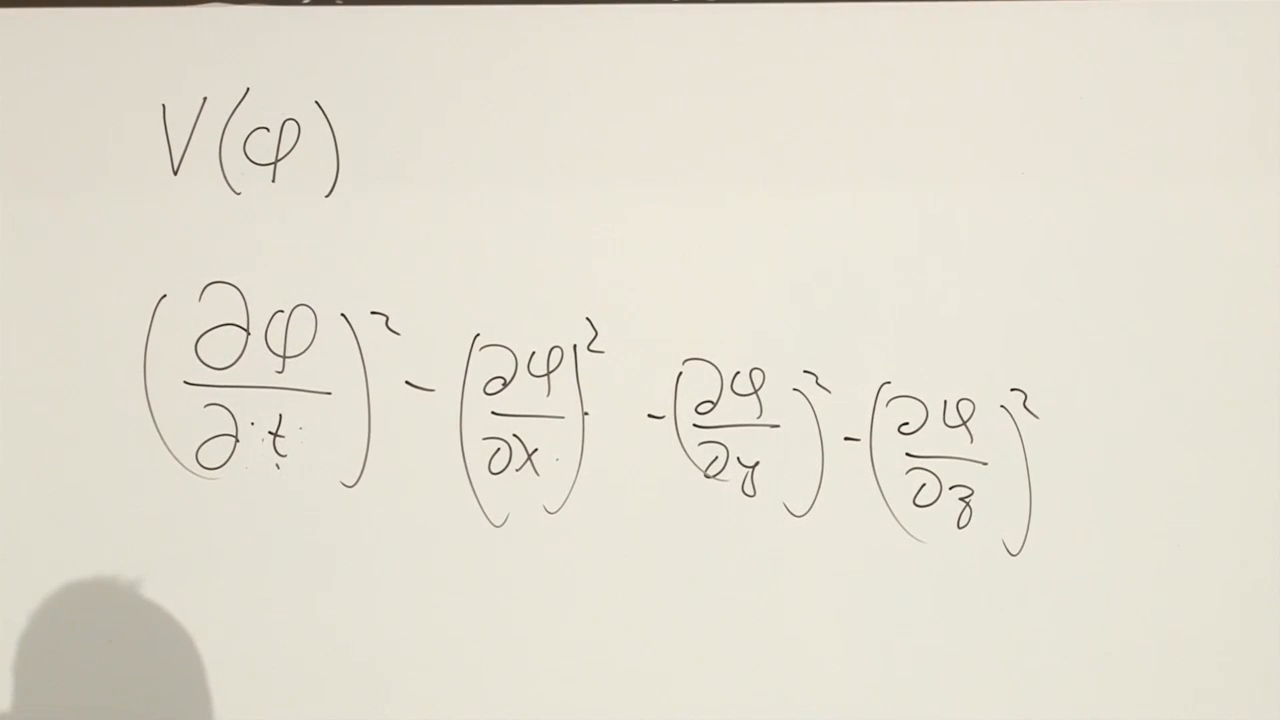
\includegraphics[width=0.90\textwidth]{lecture_04_figure_13.png}
\caption{由标量场的一阶导数构造的不变平方差。}
\lectureframe{01:13:55}
\end{figure}

\begin{classroomqa}
\audiencequestion{这个导数组合是拉普拉斯算子吗？}
\lecturerresponse{不是。所展示的不变量对一阶导数是二次的。拉普拉斯算子包含二阶空间导数。二阶导数只有在变分作用量之后、在波动方程中才会出现。\lecturetimestamp{01:13:22}}
\end{classroomqa}

\eqref{eq:sr4-scalar-lagrangian} 中的符号模式现在得到了解释，而不是猜测。动能梯度组合是洛伦兹标量
\(\partial_\mu\phi\,\partial^\mu\phi\)。因此最简单的二次理论是
\begin{equation}
\mathcal{L}
=
\frac12\partial_\mu\phi\,\partial^\mu\phi
-\frac12\mu^2\phi^2.
\label{eq:sr4-covariant-lagrangian}
\end{equation}

\begin{figure}[htbp]
\centering
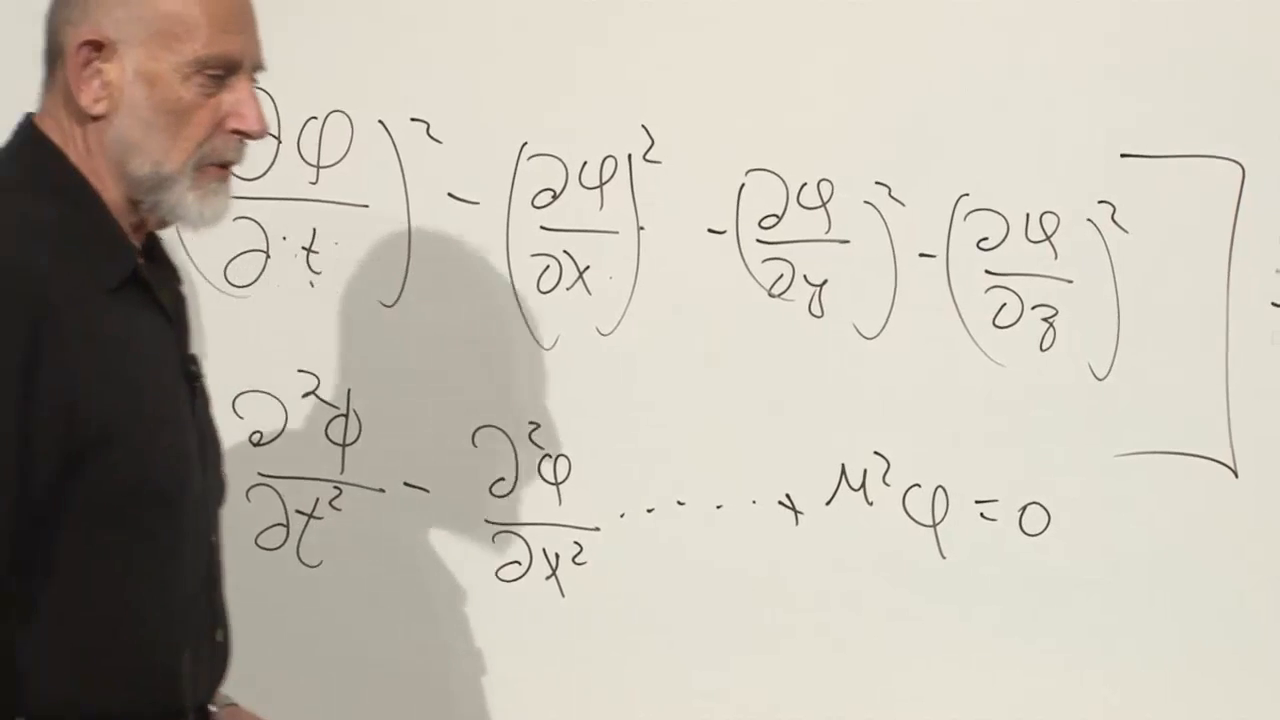
\includegraphics[width=0.90\textwidth]{lecture_04_figure_14.png}
\caption{黑板上完整的二次标量场拉格朗日量及其线性场方程。}
\lectureframe{01:19:12}
\end{figure}

\section{有多大的自由度？}

一旦知道了构造标量的规则，许多拉格朗日量就成为可能。场 \(\phi\) 是一个标量，因此每一个普通函数 \(F(\phi)\) 也是标量：\(\phi^2\)、\(\phi^3\)、\(\cosh\phi\) 等等。数值参数也是允许的。像 \(\mu\) 这样的符号可以作为常数系数插入；剩下的唯一问题是它的量纲和物理解释。

\begin{classroomqa}
\audiencequestion{可以把质量放进拉格朗日量吗？}
\lecturerresponse{常数参数当然可以。在这个阶段，人们应当问它是哪个物体的质量，因为在经典场论中，\(\mu\) 在确定其物理意义之前只是一个数。在二次相对论标量理论中，它设定了质量或长度倒数的标度。\lecturetimestamp{01:14:16}}
\end{classroomqa}

标量可以相乘：
\begin{equation}
F(\phi)\,\partial_\mu\phi\,\partial^\mu\phi
\end{equation}
是洛伦兹不变的。导数标量本身也可以平方，从而产生一阶导数的更高次幂。人们也可以考虑更高阶导数，尽管本讲义将注意力限制在场及其一阶导数上，这是产生二阶运动方程的标准框架。高阶导数理论需要额外的谨慎，因为它们一般会引入额外的动力学数据和可能的不稳定性。

\begin{classroomqa}
\audiencequestion{平方差构造真的是时空的度规吗？}
\lecturerresponse{是的。在所选取的号差下，度规是 \(dt^2-dx^2-dy^2-dz^2\)。讲义尚未强调度规这个词，但这正是将在广义相对论中成为核心的时空几何。\lecturetimestamp{01:19:39}}
\end{classroomqa}

\begin{classroomqa}
\audiencequestion{是否存在比四维矢量更一般的对象，其分量如 \(xy\) 或 \(tx\)？}
\lecturerresponse{是的。那些是张量。标量没有时空指标，矢量有一个指标，而二阶张量的分量如 \(T^{xx}\)、\(T^{xy}\) 和 \(T^{tx}\)。目前关于标量场的讨论大多避开了它们；在广义相对论中它们将不可避免。\lecturetimestamp{01:20:49}}
\end{classroomqa}

\begin{classroomqa}
\audiencequestion{为什么只讨论将 \(t\) 与 \(x\) 混合的助推？助推能否指向另一个方向，并以不同方式混合空间轴？}
\lecturerresponse{当然可以。沿 \(y\) 方向的助推将 \(t\) 与 \(y\) 混合，并保持 \(x,z\) 不变。一般的洛伦兹变换可以由空间旋转和沿选定轴的助推组合而成。因此，只需确立旋转不变性以及沿一个标准轴的助推下的不变性就足够了。\lecturetimestamp{01:22:06}}
\end{classroomqa}

\begin{classroomqa}
\audiencequestion{面对如此多可能的标量组合，所有由此得到的拉格朗日量都描述有意义的物理吗？}
\lecturerresponse{在经典层面，这种自由度是巨大的，但受制于诸如符号合理、局域性以及演化问题适定等附加要求。定义行为良好的基本量子理论所需的任意选择要少得多。现代有效场论允许在截断尺度以下存在许多附加相互作用，但此时必须说明其有效范围。\lecturetimestamp{01:27:57}}
\end{classroomqa}

\begin{classroomqa}
\audiencequestion{场必须是连续的吗？}
\lecturerresponse{对于所讨论的光滑理论，是的。跳跃会产生奇异的导数，并且在有二次梯度项时，通常会导致作用量和能量发散。更奇异的位形只能借助额外的数学结构来处理；它们不是这里所发展的普通有限能量场。\lecturetimestamp{01:29:29}}
\end{classroomqa}

\section{粒子与标量场的耦合}

\subsection{重新审视自由粒子}

讲座的最后一部分在经典层面将粒子与场结合起来。这还不是粒子是场的激发的量子陈述。相反，假设已经有人解出了背景标量场\(\phi(x,t)\)，并询问粒子如何在其中运动。

对于自由相对论粒子，
\begin{equation}
A_{\rm free}=-m\int d\tau.
\label{eq:sr4-free-particle-action}
\end{equation}
在一维空间且\(c=1\)时，
\begin{equation}
d\tau=dt\sqrt{1-\dot x^2},
\qquad
L_{\rm free}=-m\sqrt{1-\dot x^2}.
\label{eq:sr4-free-particle-l}
\end{equation}
选择负号是为了使低速展开给出通常的正牛顿动能项：
\begin{equation}
L_{\rm free}
\approx -m+\frac12m\dot x^2+\cdots.
\end{equation}

\begin{figure}[htbp]
\centering
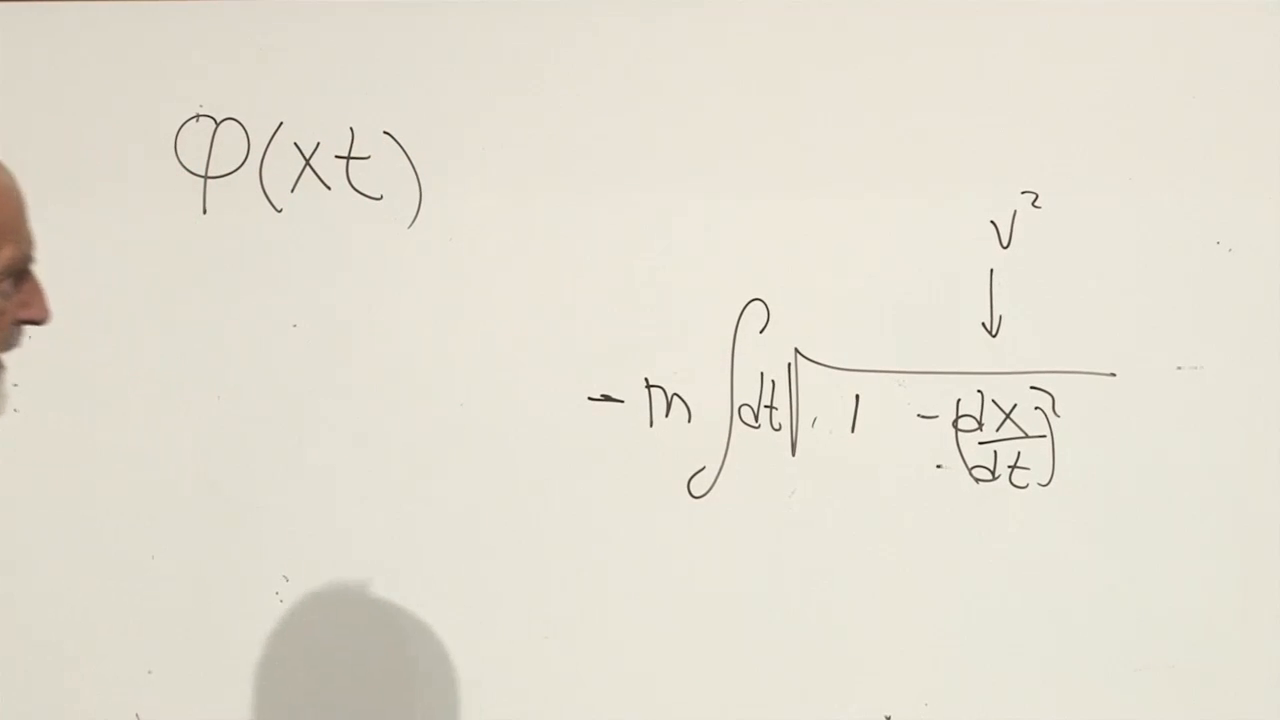
\includegraphics[width=0.90\textwidth]{lecture_04_figure_15.png}
\caption{将不变的自由粒子作用量改写为坐标时间拉格朗日量。}
\lectureframe{01:34:31}
\end{figure}

\subsection{最简单的标量耦合}

\(d\tau\)和\(\phi\)都是标量。因此最简单的线性耦合是
\begin{equation}
\boxed{
A
=
\int d\tau\,[-m+\phi(x,t)]
}.
\label{eq:sr4-coupled-action}
\end{equation}
这一选择并不唯一。可以用任意函数\(F(\phi)\)替换\(\phi\)。线性项已足以展示物理思想。

\begin{figure}[htbp]
\centering
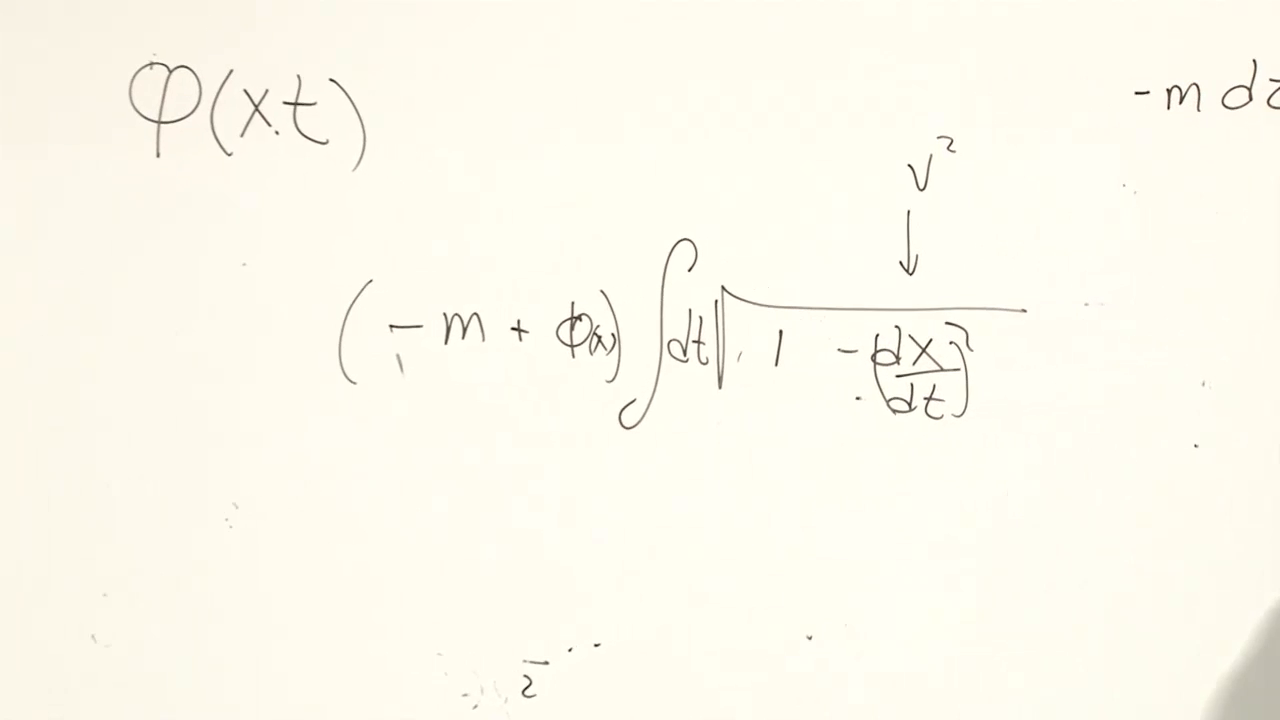
\includegraphics[width=0.90\textwidth]{lecture_04_figure_16.png}
\caption{自由作用量加上最简单的洛伦兹不变标量耦合。}
\lectureframe{01:37:21}
\end{figure}

\begin{classroomqa}
\audiencequestion{\(\phi\)必须留在积分内吗？}
\lecturerresponse{是的。场是在粒子的世界线上\(\phi(x(t),t)\)取值的，并且一般会从轨迹的一点到另一点发生变化。即使背景没有显式的时间依赖，\(\phi=\phi(x)\)，当粒子在空间中运动时，它仍然随时间变化。只有沿路径恒定的场才能被提到积分外。\lecturetimestamp{01:37:47}}
\end{classroomqa}

\begin{classroomqa}
\audiencequestion{\(\phi(x,t)\)中的\(x\)表示粒子的位置吗？}
\lecturerresponse{是的。它是\(x=x(t)\)，即粒子在时刻\(t\)的位置。作用量沿该轨迹对给定的时空场进行采样。\lecturetimestamp{01:38:08}}
\end{classroomqa}

对于一维运动，\eqref{eq:sr4-coupled-action}给出
\begin{equation}
L
=
-(m-\phi(x,t))\sqrt{1-\dot x^2}.
\label{eq:sr4-coupled-lagrangian}
\end{equation}
标量背景恰好出现在静质量所占据的位置：
\begin{equation}
m_{\rm eff}(x,t)=m-\phi(x,t).
\label{eq:sr4-effective-mass}
\end{equation}
如果\(\phi\)趋于一个近似恒定的非零值，粒子的行为就好像其质量发生了移动。这只是一个经典玩具模型，不是完整的希格斯机制，但它捕捉到了所宣传的希格斯思想的意味：标量背景可以作为质量项进入粒子动力学。

\subsection{粒子方程}

正则动量为
\begin{equation}
p
=
\frac{\partial L}{\partial\dot x}
=
(m-\phi)
\frac{\dot x}{\sqrt{1-\dot x^2}}.
\label{eq:sr4-coupled-momentum}
\end{equation}

\begin{figure}[htbp]
\centering
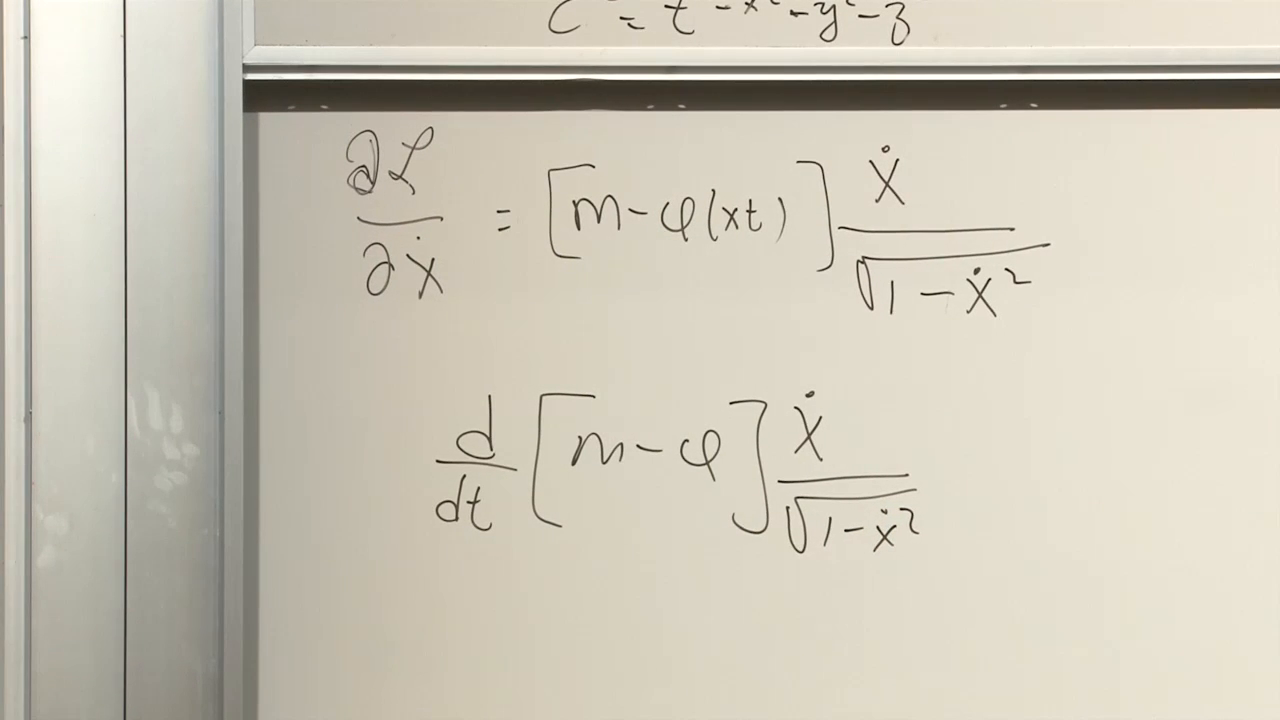
\includegraphics[width=0.90\textwidth]{lecture_04_figure_17.png}
\caption{标量背景在相对论正则动量中将\(m\)替换为\(m-\phi(x,t)\)。}
\lectureframe{01:43:38}
\end{figure}

拉格朗日量对位置的导数为
\begin{equation}
\frac{\partial L}{\partial x}
=
\frac{\partial\phi}{\partial x}
\sqrt{1-\dot x^2}.
\end{equation}
由作用量\eqref{eq:sr4-coupled-action}固定符号后，欧拉--拉格朗日方程因此为
\begin{equation}
\boxed{
\frac{d}{dt}
\left[
(m-\phi)
\frac{\dot x}{\sqrt{1-\dot x^2}}
\right]
=
\frac{\partial\phi}{\partial x}
\sqrt{1-\dot x^2}
}.
\label{eq:sr4-coupled-eom}
\end{equation}

\begin{figure}[htbp]
\centering
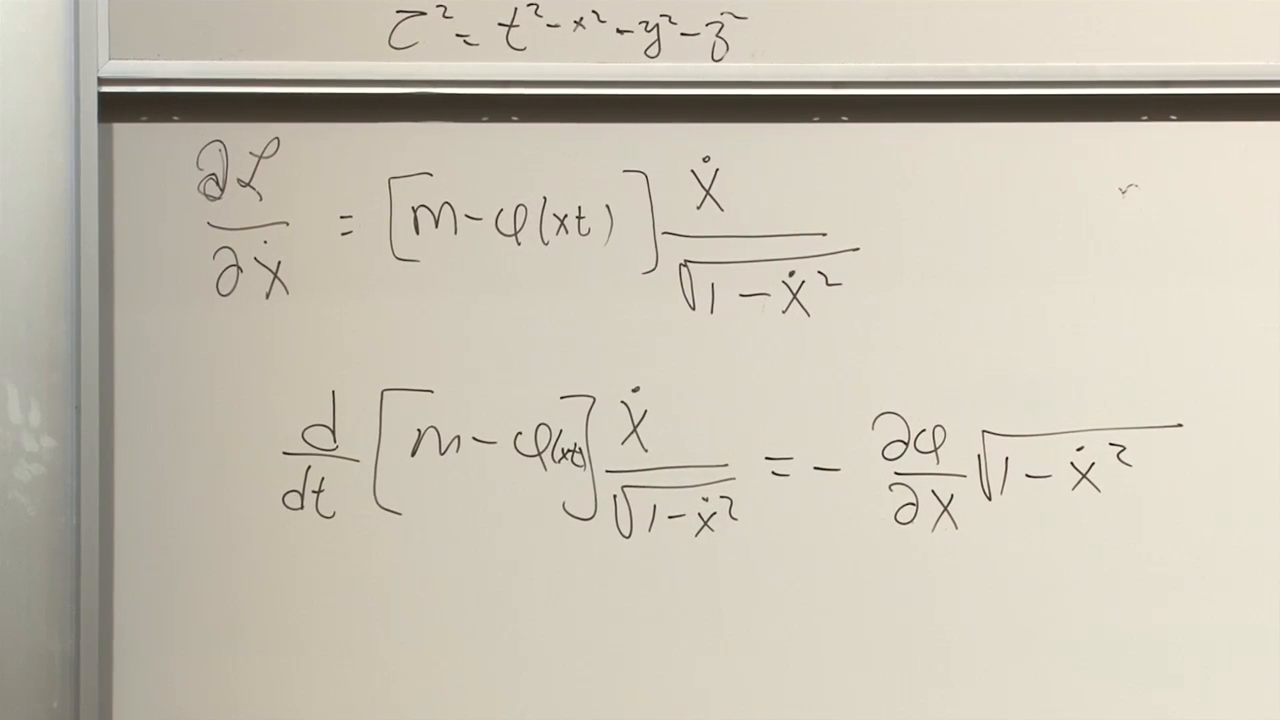
\includegraphics[width=0.90\textwidth]{lecture_04_figure_18.png}
\caption{耦合方程由动量和背景场的空间导数组装而成；作用量确定了\eqref{eq:sr4-coupled-eom}中的最终符号。}
\lectureframe{01:45:24}
\end{figure}

\begin{classroomqa}
\audiencequestion{为什么\(\partial\phi/\partial x\)保留因子\(\sqrt{1-\dot x^2}\)？}
\lecturerresponse{因为只有因子\(\phi(x,t)\)对\(x\)求导。在拉格朗日量中平方根乘在它前面，并且当\(\dot x\)在偏导数中保持固定时，平方根与位置无关，所以平方根保留下来。\lecturetimestamp{01:45:50}}
\end{classroomqa}

展开全时间导数得到
\begin{align}
&(m-\phi)
\frac{d}{dt}
\left(
\frac{\dot x}{\sqrt{1-\dot x^2}}
\right)
-
\dot\phi\,
\frac{\dot x}{\sqrt{1-\dot x^2}}
\nonumber\\
&\hspace{10em}
=
\frac{\partial\phi}{\partial x}
\sqrt{1-\dot x^2}.
\label{eq:sr4-coupled-expanded}
\end{align}
如果背景是静态的，\(\phi=\phi(x)\)，它沿运动世界线的导数并不为零。链式法则给出
\begin{equation}
\boxed{
\dot\phi
=
\frac{d}{dt}\phi(x(t))
=
\frac{\partial\phi}{\partial x}\dot x
}.
\label{eq:sr4-chain-rule}
\end{equation}

\begin{classroomqa}
\audiencequestion{如果\(\phi\)没有显式的时间依赖，为什么\(\dot\phi\)不为零？}
\lecturerresponse{因为粒子改变了位置。场是在\(x(t)\)处取样的，所以它的全导数是\(\dot\phi=\phi_x\dot x\)。静态场意味着\(\partial\phi/\partial t=0\)，而不是每个运动的粒子都看到恒定的场值。\lecturetimestamp{01:48:10}}
\end{classroomqa}

\begin{figure}[htbp]
\centering
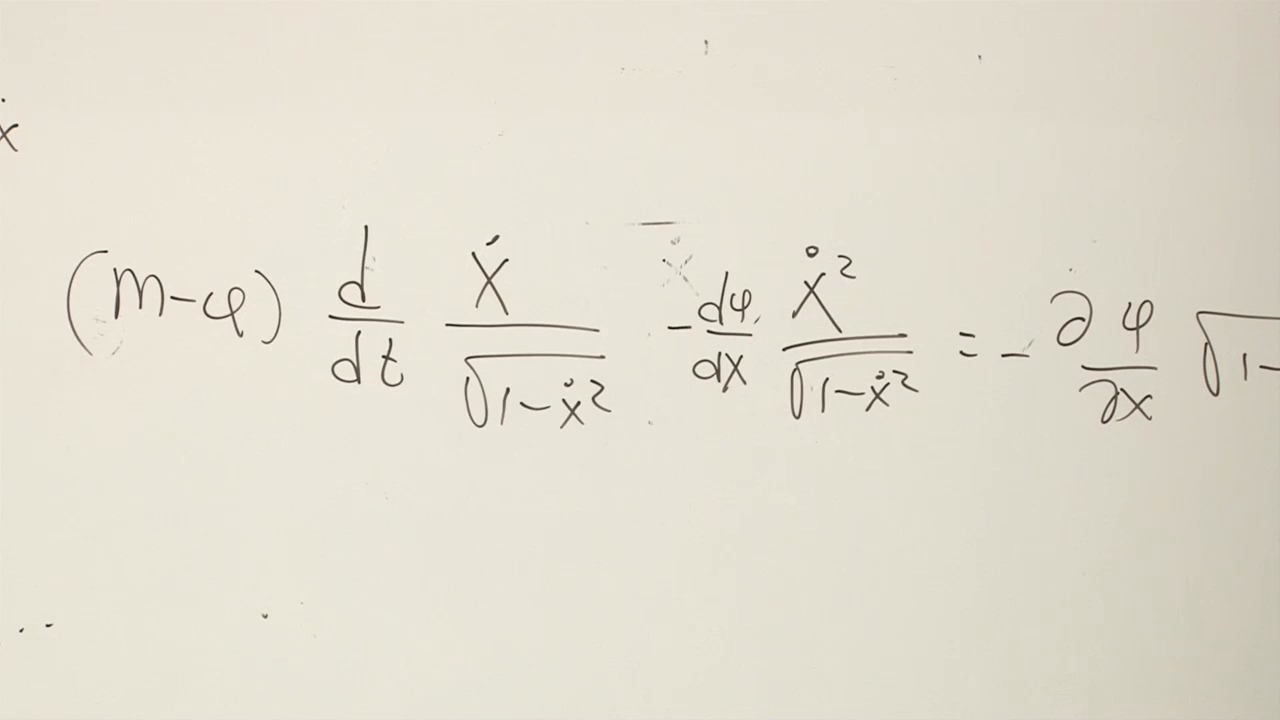
\includegraphics[width=0.90\textwidth]{lecture_04_figure_19.png}
\caption{沿世界线使用链式法则后，耦合方程的后段展开。}
\lectureframe{01:49:11}
\end{figure}

精确表达式并不特别漂亮，讲座也不假装它漂亮。然而它的慢速极限却是熟悉的。由于\(\sqrt{1-\dot x^2}\approx1\)，领头方程为
\begin{equation}
\frac{d}{dt}\bigl[(m-\phi)\dot x\bigr]
\approx
\frac{\partial\phi}{\partial x}.
\end{equation}
如果有效质量的变化也作微扰处理，这就变成
\begin{equation}
(m-\phi)\ddot x
\approx
\frac{\partial\phi}{\partial x}.
\label{eq:sr4-nonrel-force}
\end{equation}
的确，低速拉格朗日量为
\begin{equation}
L
\approx
-m+\phi+\frac12(m-\phi)\dot x^2,
\end{equation}
所以在领头阶，势能是\(U=-\phi\)，力是\(-dU/dx=\partial_x\phi\)。恢复\(c\)的因子并重现这一牛顿力学模式，就是讲座结束时留下的练习。

从粒子到场的路径现在完整了。粒子历史\(\phi(t)\)提供了\(0+1\)维的原型；场历史\(\phi(x)\)把作用量提升为时空积分；场的欧拉--拉格朗日方程产生了波动动力学；洛伦兹标量选出了相对论性的符号结构；而同样的不变量语言让标量背景能够反过来作用于粒子。
